\section{mr::sampler Struct Reference}
\label{structmr_1_1sampler}\index{mr::sampler@{mr::sampler}}
{\tt \#include $<$mr\-Sampler.h$>$}

Inheritance diagram for mr::sampler::\begin{figure}[H]
\begin{center}
\leavevmode
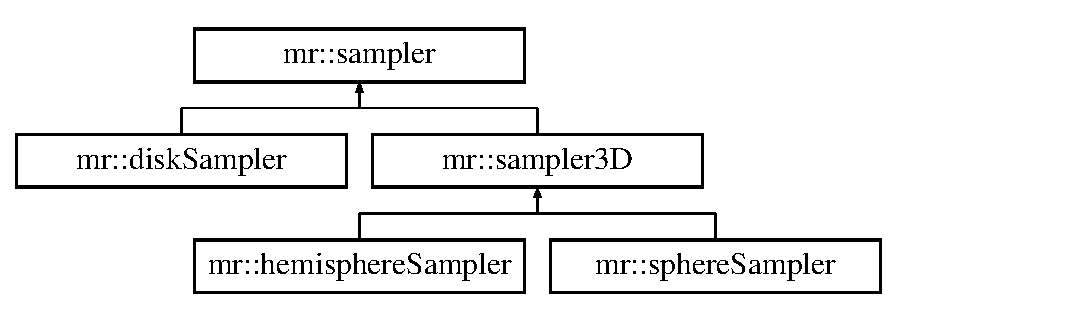
\includegraphics[height=3cm]{structmr_1_1sampler}
\end{center}
\end{figure}
\subsection*{Public Member Functions}
\begin{CompactItemize}
\item 
{\bf sampler} ()
\begin{CompactList}\small\item\em Constructor for adaptive sampling. \item\end{CompactList}\item 
{\bf sampler} (const mi\-Uint \&num\-Samples)
\begin{CompactList}\small\item\em Constructor for fixed sampling. num\-Samples HAS to be mi\-Uint\&. \item\end{CompactList}\item 
{\bf $\sim$sampler} ()
\item 
const int {\bf count} ()
\begin{CompactList}\small\item\em Returns the number of samples taken so far. \item\end{CompactList}\end{CompactItemize}
\subsection*{Public Attributes}
\begin{CompactItemize}
\item 
const mi\-Uint $\ast$ {\bf max\-Samples}
\item 
int {\bf counter}
\end{CompactItemize}


\subsection{Constructor \& Destructor Documentation}
\index{mr::sampler@{mr::sampler}!sampler@{sampler}}
\index{sampler@{sampler}!mr::sampler@{mr::sampler}}
\subsubsection{\setlength{\rightskip}{0pt plus 5cm}mr::sampler::sampler ()\hspace{0.3cm}{\tt  [inline]}}\label{structmr_1_1sampler_a0}


Constructor for adaptive sampling. 

\index{mr::sampler@{mr::sampler}!sampler@{sampler}}
\index{sampler@{sampler}!mr::sampler@{mr::sampler}}
\subsubsection{\setlength{\rightskip}{0pt plus 5cm}mr::sampler::sampler (const mi\-Uint \& {\em num\-Samples})\hspace{0.3cm}{\tt  [inline]}}\label{structmr_1_1sampler_a1}


Constructor for fixed sampling. num\-Samples HAS to be mi\-Uint\&. 

\index{mr::sampler@{mr::sampler}!~sampler@{$\sim$sampler}}
\index{~sampler@{$\sim$sampler}!mr::sampler@{mr::sampler}}
\subsubsection{\setlength{\rightskip}{0pt plus 5cm}mr::sampler::$\sim${\bf sampler} ()\hspace{0.3cm}{\tt  [inline]}}\label{structmr_1_1sampler_a2}




\subsection{Member Function Documentation}
\index{mr::sampler@{mr::sampler}!count@{count}}
\index{count@{count}!mr::sampler@{mr::sampler}}
\subsubsection{\setlength{\rightskip}{0pt plus 5cm}const int mr::sampler::count ()\hspace{0.3cm}{\tt  [inline]}}\label{structmr_1_1sampler_a3}


Returns the number of samples taken so far. 



\subsection{Member Data Documentation}
\index{mr::sampler@{mr::sampler}!counter@{counter}}
\index{counter@{counter}!mr::sampler@{mr::sampler}}
\subsubsection{\setlength{\rightskip}{0pt plus 5cm}int {\bf mr::sampler::counter}}\label{structmr_1_1sampler_o1}


\index{mr::sampler@{mr::sampler}!maxSamples@{maxSamples}}
\index{maxSamples@{maxSamples}!mr::sampler@{mr::sampler}}
\subsubsection{\setlength{\rightskip}{0pt plus 5cm}const mi\-Uint$\ast$ {\bf mr::sampler::max\-Samples}}\label{structmr_1_1sampler_o0}




The documentation for this struct was generated from the following file:\begin{CompactItemize}
\item 
{\bf mr\-Sampler.h}\end{CompactItemize}
